\chapter{Avaliação dos Modelos de Aprendizado de Máquina (AM)}

Este capítulo apresenta os resultados obtidos a partir da aplicação dos modelos de Aprendizado de Máquina desenvolvidos neste trabalho. 
Inicialmente, são discutidas as métricas de desempenho alcançadas pelos modelos na tarefa de predição da pontuação final das equipes. 
Em seguida, é realizada uma análise do comportamento das previsões, buscando avaliar a capacidade dos modelos em capturar padrões relevantes a partir das estatísticas 
individuais dos jogadores.

\section{Modelos de Aprendizado de Máquina (AM)}

Como referência para interpretação dos resultados, considera-se o modelo de baseline implícito associado
ao coeficiente de determinação. Em problemas de regressão, um valor de $R^2 = 0$ corresponde a um modelo
que simplesmente prevê a média da variável alvo para todas as observações, isto é, a pontuação média
dos clubes na liga. Dessa forma, valores positivos de $R^2$ indicam que o modelo consegue explicar parte
da variabilidade observada nos dados, superando a estratégia trivial de prever sempre a média das pontuações.

O melhor modelo de AM desenvolvido neste estudo apresentou um coeficiente de determinação máximo de
aproximadamente $0{,}55$ na tarefa de prever a pontuação final de um time em sua liga nacional, utilizando
como base os dados estatísticos de desempenho individual de seus jogadores na temporada anterior.

Para avaliar o desempenho dos diferentes algoritmos aplicados à tarefa de previsão, foram calculadas métricas 
amplamente utilizadas em problemas de regressão, incluindo o coeficiente de determinação (R\textsuperscript{2}), 
o erro absoluto médio (MAE), o erro quadrático médio (MSE), a raiz do erro quadrático médio (RMSE), 
o erro percentual absoluto médio (MAPE) e o tempo de processamento de cada modelo. A Tabela~\ref{tab:comparacao_modelos} 
apresenta um resumo comparativo dos resultados obtidos, permitindo analisar tanto a qualidade preditiva 
quanto o custo computacional de cada abordagem.

\begin{table}[H]
\centering
\caption{Comparação de desempenho entre os modelos de Machine Learning avaliados no conjunto de testes}
\label{tab:comparacao_modelos}

\begin{tabular}{lcccccc}
\hline
\textbf{Modelo} & \textbf{R\textsuperscript{2}} & \textbf{MAE} & \textbf{MSE} & \textbf{RMSE} & \textbf{MAPE} & \textbf{Tempo (s)} \\
\hline
RL      & 0,41 & 11,48 & 191,78 & 13,85 & 0,2580 & 1,72 \\
RF      & 0,46 & 10,52 & 174,98 & 13,23 & 0,2390 & 118,66 \\
XGBoost & 0,41 & 11,23 & 191,23 & 13,83 & 0,2512 & 99,08 \\
MLP     & 0,55 & 11,08 & 170,42 & 13,05 & 0,2424 & 161,68 \\
\hline
\end{tabular}

\vspace{.3cm}
\fonte{Elaborado pelo autor.}
\end{table}

Os resultados apresentados na Tabela~\ref{tab:comparacao_modelos} evidenciam um desempenho moderado dos algoritmos avaliados na tarefa de previsão da 
pontuação final dos clubes. O melhor modelo alcançou um valor de $R^2$ de aproximadamente $0{,}55$, indicando que parte significativa da variabilidade 
da pontuação pode ser explicada pelas variáveis consideradas, embora ainda exista um grau relevante de incerteza inerente ao problema. A pontuação de um time 
ao longo de uma temporada é influenciada por diversos fatores não diretamente capturados pelas estatísticas individuais dos jogadores, como aspectos táticos, 
mudanças de treinador, lesões, dinâmica coletiva e variações contextuais ao longo do campeonato, o que naturalmente impõe um limite ao desempenho preditivo dos modelos.

Entre os métodos avaliados, a Rede Neural Multicamadas (MLP) apresentou o melhor desempenho geral. O modelo obteve o maior valor de $R^2$ (0{,}55), além dos 
menores valores de MSE e RMSE, indicando maior capacidade de capturar a variabilidade presente nos dados. Esses resultados sugerem que a arquitetura neural foi 
mais eficaz em explorar relações não lineares existentes entre os componentes principais gerados pelo PCA e a pontuação final das equipes.

O modelo de \textit{Random Forest} apresentou o segundo melhor desempenho, alcançando $R^2$ de 0{,}46 e os menores valores de MAE e MAPE entre os 
modelos avaliados. Esse resultado indica que o método baseado em árvores também foi capaz de capturar padrões relevantes nos dados, embora com menor 
capacidade explicativa global em comparação à MLP. Ainda assim, o custo computacional do RF foi significativamente inferior ao da rede neural, o que pode 
torná-lo uma alternativa interessante em cenários em que o tempo de treinamento seja um fator crítico.

Por outro lado, os modelos de Regressão Linear (RL) e \textit{XGBoost} apresentaram desempenhos bastante semelhantes entre si, ambos com $R^2$ em torno de 0{,}41 
e erros superiores aos observados nos demais métodos. Esse comportamento sugere que, embora parte da variabilidade da pontuação possa ser explicada por relações 
aproximadamente lineares entre os componentes principais e a variável alvo, a presença de padrões não lineares limita a capacidade desses modelos de alcançar 
desempenhos superiores nesse contexto.

De maneira geral, os resultados indicam que modelos capazes de capturar relações não lineares mais complexas tendem a apresentar melhor desempenho na tarefa 
considerada. Dessa forma, o MLP foi selecionado como modelo preditivo para as etapas subsequentes do estudo.

\subsection{Predição do Modelo Multilayer Perceptron (MLP)}

Antes de analisar as previsões realizadas pelo modelo, foi avaliado o comportamento do processo de treinamento da rede neural ao longo das épocas. 
A Figura~\ref{fig:mlp_mae} apresenta a evolução do erro absoluto médio (MAE) durante o treinamento da rede MLP, considerando tanto o conjunto de 
treinamento quanto o conjunto de validação.

\begin{figure}[H]
\centering
\caption{Evolução do erro absoluto médio (MAE) ao longo das épocas de treinamento da rede MLP para os conjuntos de treinamento e validação.}
\label{fig:mlp_mae}

\includegraphics[width=0.9\textwidth]{imagens/mlp_mae.png}
\fonte{Elaborado pelo autor.}
\end{figure}

Observa-se uma redução acentuada do erro nas primeiras épocas de treinamento, indicando que o modelo rapidamente aprende padrões relevantes presentes nos dados. 
Após essa fase inicial, o erro tende a estabilizar, apresentando pequenas oscilações ao longo das épocas subsequentes.

Nota-se também que as curvas de treinamento e validação permanecem relativamente próximas durante todo o processo de treinamento, sugerindo ausência de 
sobreajuste significativo (\textit{overfitting}). Esse comportamento indica que o modelo manteve boa capacidade de generalização ao longo do treinamento.

Com o intuito de compreender a predição realizada pelo melhor modelo (MLP), foi realizada uma análise visual da relação entre as pontuações reais dos 
clubes da Premier League e as pontuações previstas pelo modelo ao longo das temporadas analisadas.

As Figuras~\ref{fig:pl_20_21}--\ref{fig:pl_23_24} apresentam os gráficos de comparação entre as pontuações reais e previstas pelo modelo MLP para 
as temporadas de 2020--2021 a 2023--2024 da Premier League.

\begin{figure}[H]
\centering
\caption{Comparação entre pontuações reais e previstas pelo modelo MLP na temporada 2020--2021 da Premier League.}
\label{fig:pl_20_21}
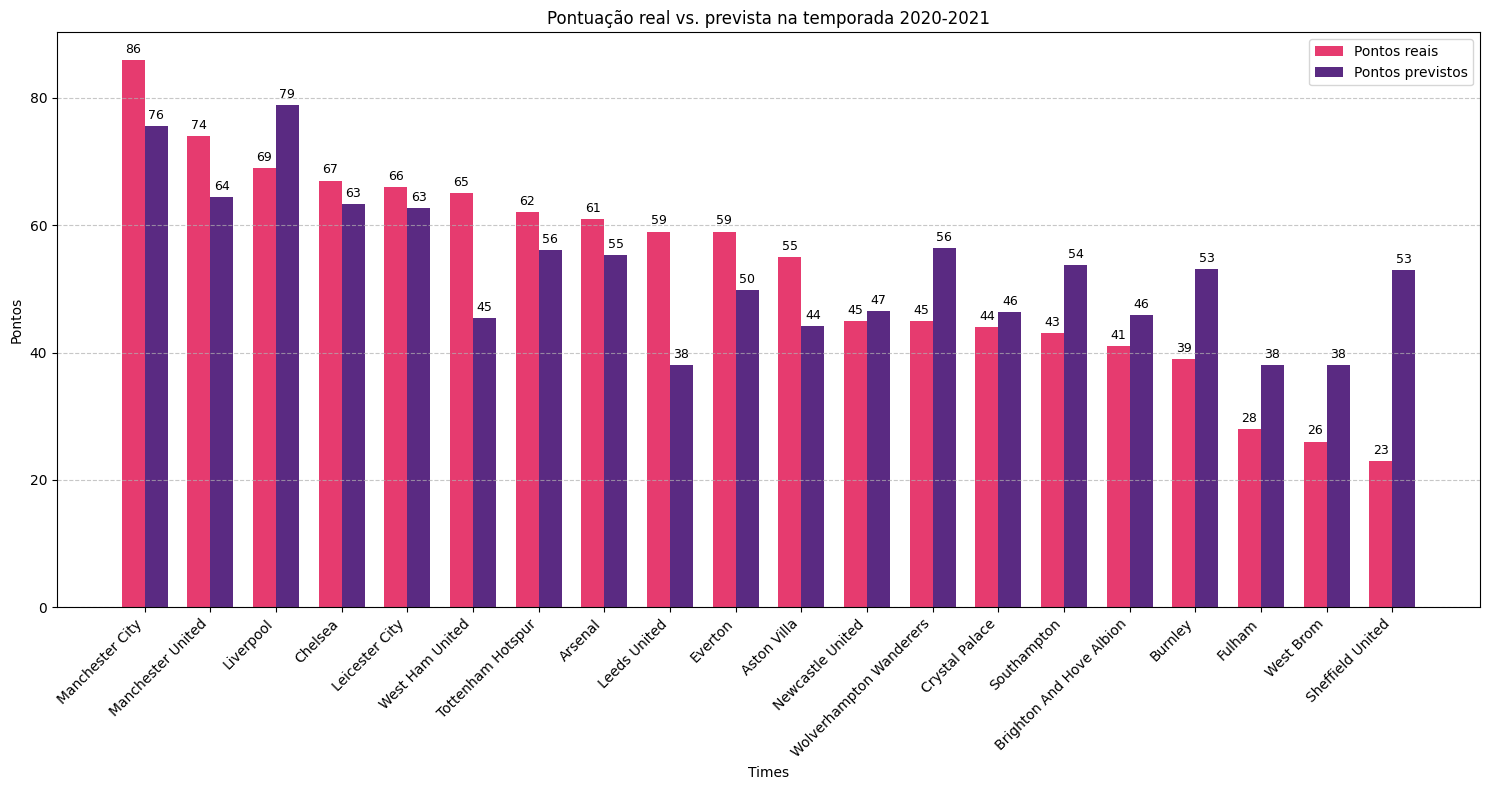
\includegraphics[width=\textwidth]{imagens/pl_20-21.png}
\fonte{Elaborado pelo autor.}
\end{figure}

\begin{figure}[H]
\centering
\caption{Comparação entre pontuações reais e previstas pelo modelo MLP na temporada 2021--2022 da Premier League.}
\label{fig:pl_21_22}
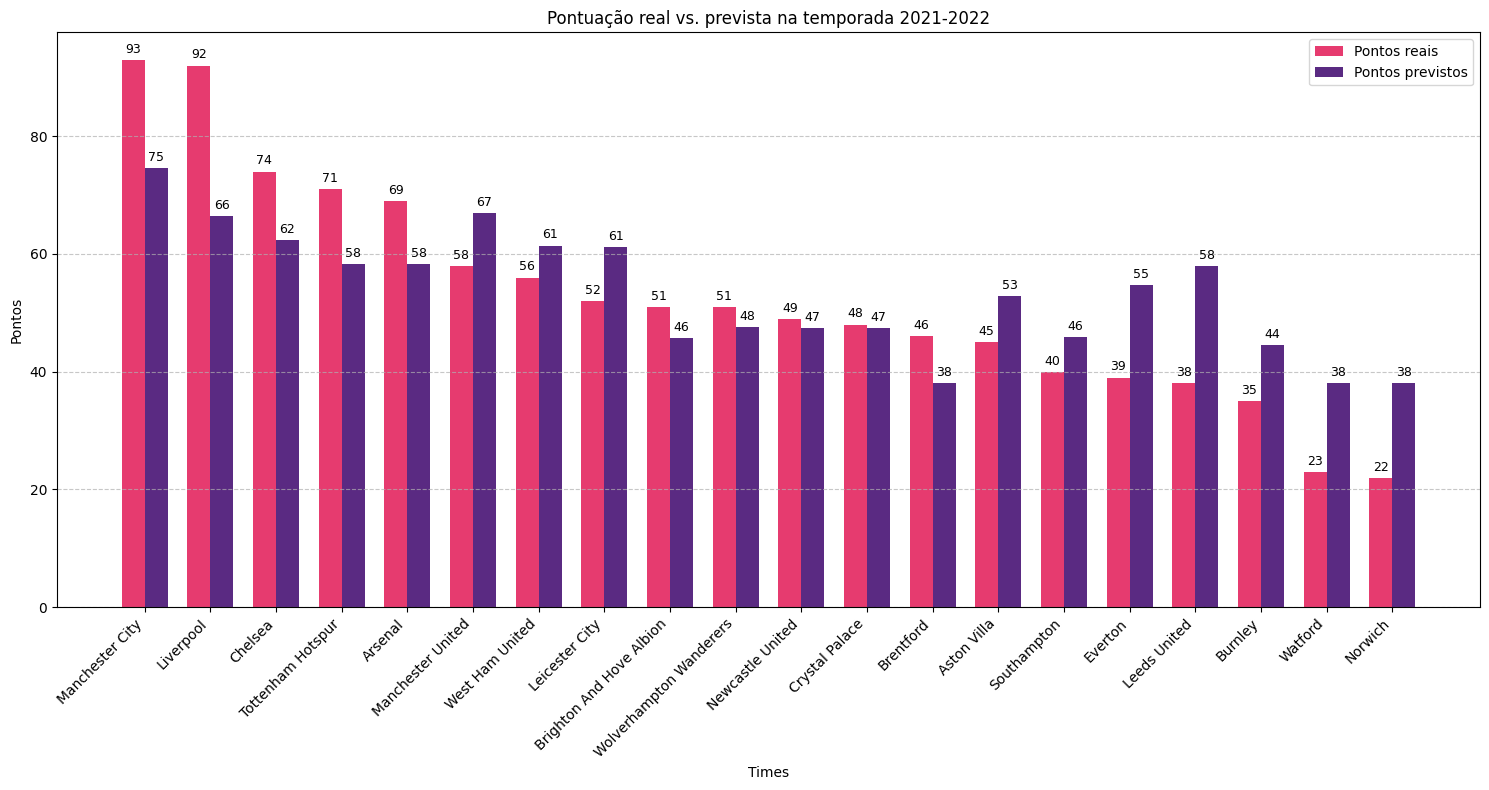
\includegraphics[width=\textwidth]{imagens/pl_21-22.png}
\fonte{Elaborado pelo autor.}
\end{figure}

\begin{figure}[H]
\centering
\caption{Comparação entre pontuações reais e previstas pelo modelo MLP na temporada 2022--2023 da Premier League.}
\label{fig:pl_22_23}
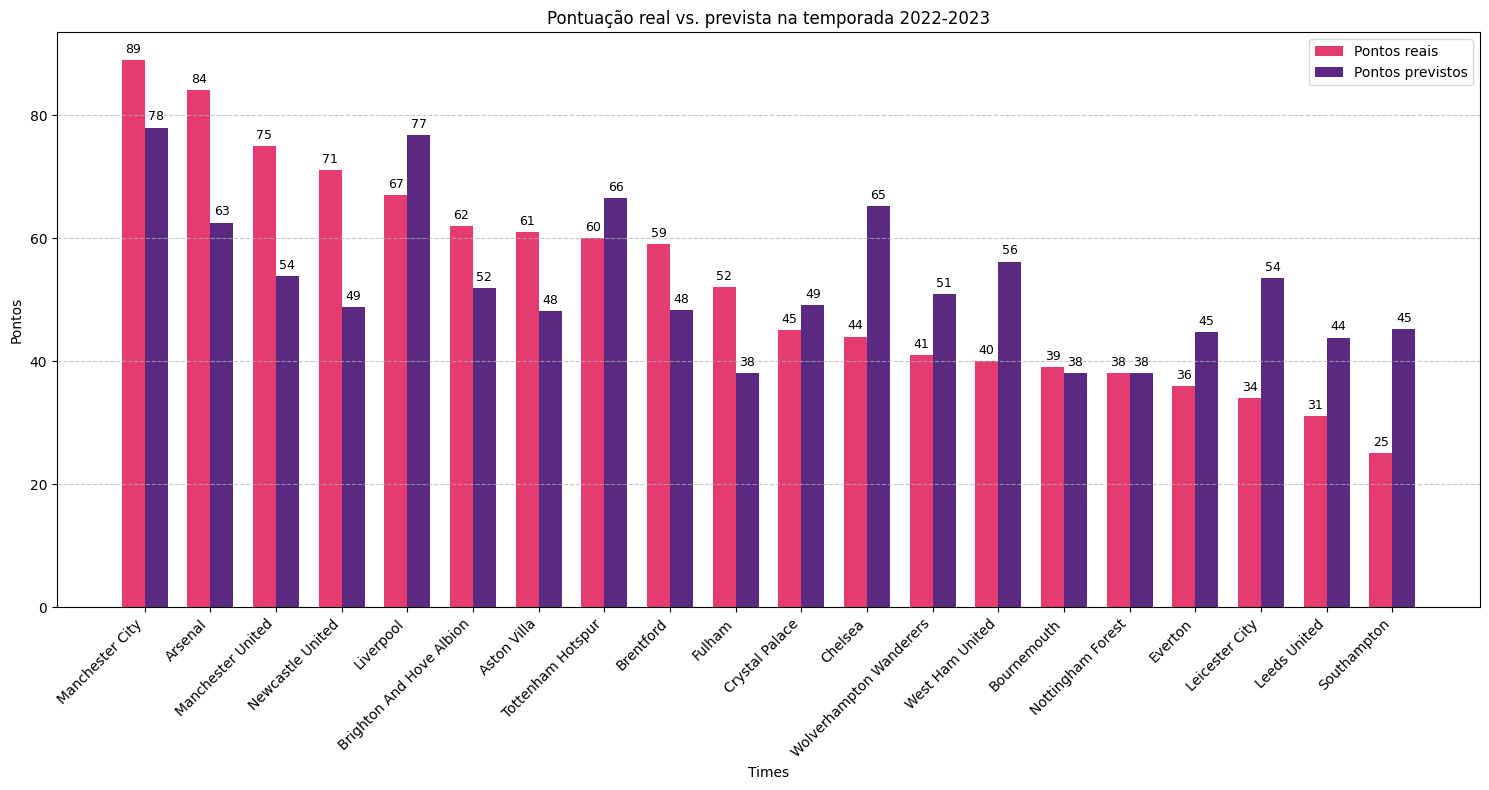
\includegraphics[width=\textwidth]{imagens/pl_22-23.png}
\fonte{Elaborado pelo autor.}
\end{figure}

\begin{figure}[H]
\centering
\caption{Comparação entre pontuações reais e previstas pelo modelo MLP na temporada 2023--2024 da Premier League.}
\label{fig:pl_23_24}
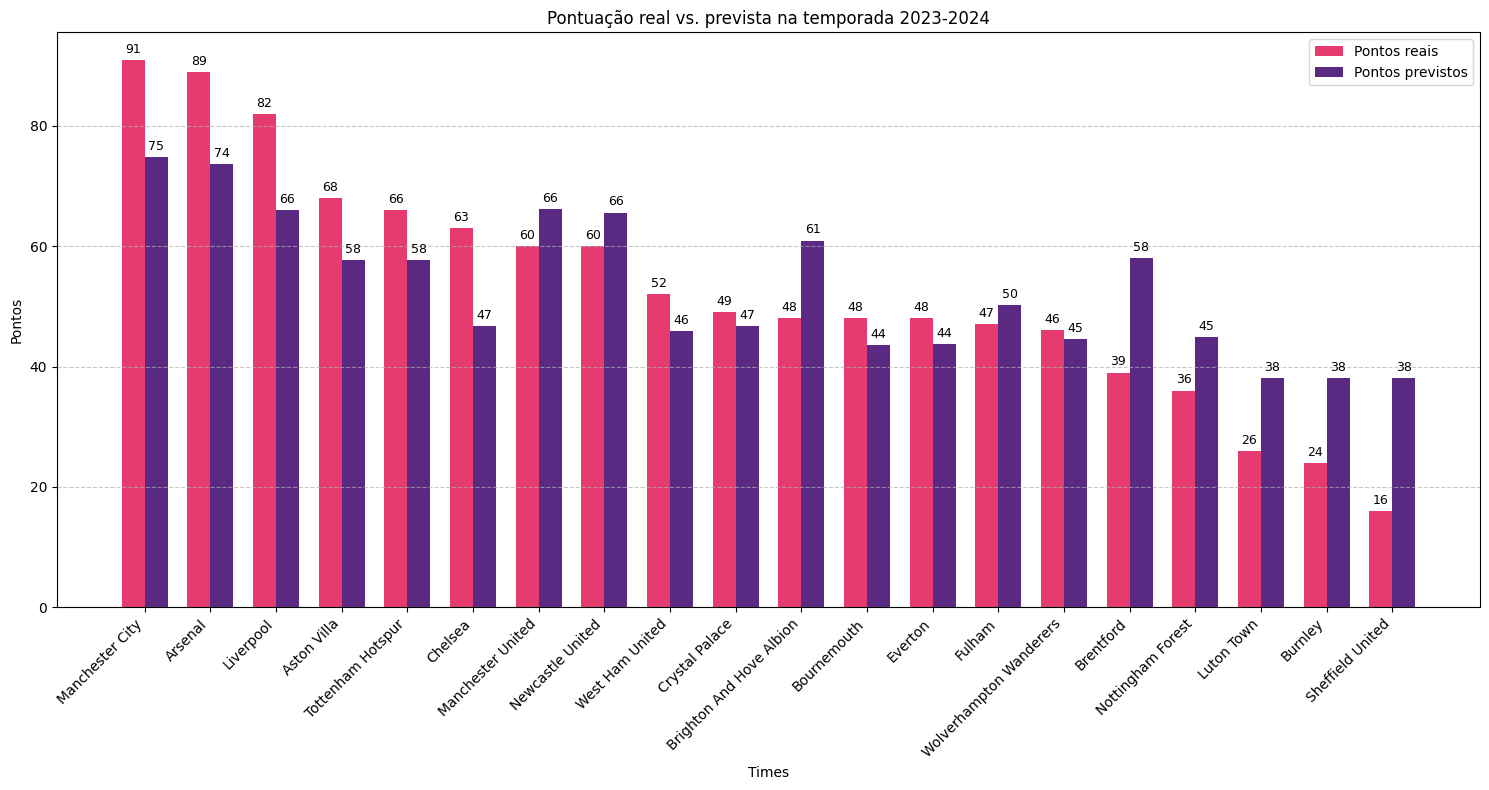
\includegraphics[width=\textwidth]{imagens/pl_23-24.png}
\fonte{Elaborado pelo autor.}
\end{figure}

Os resultados apresentados nas Figuras~\ref{fig:pl_20_21}--\ref{fig:pl_23_24} indicam que o modelo MLP apresenta maior precisão ao estimar as pontuações de 
clubes que terminaram as temporadas com valores próximos da média da liga. Clubes posicionados próximos à região central da tabela, tendem a ter suas pontuações 
previstas com menor erro. Esse comportamento é comum em modelos preditivos sob alta incerteza: quando os atributos disponíveis não capturam toda 
a variabilidade do fenômeno, as previsões convergem naturalmente para valores intermediários.

Esse resultado alinha-se com a literatura clássica, segundo a qual modelos preditivos em ambientes de alta variabilidade, como é o caso do futebol, tendem 
a gerar funções de saída menos extremas e com menor amplitude, aproximando-se de valores centrais, devido a mecanismos de \textit{shrinkage} e ao balanço 
entre viés e variância discutidos por Bishop~\cite{bishop2006}. Esse comportamento é análogo ao fenômeno estatístico conhecido como regressão à média.

Dessa forma, observa-se que o modelo MLP é capaz de capturar tendências gerais de desempenho dos clubes com base nas estatísticas individuais de seus jogadores, 
porém nota-se uma subestimação sistemática das equipes de desempenho elevado, como Manchester City, Arsenal e Liverpool, e uma superestimação das equipes de baixo 
desempenho, como Sheffield United, Burnley e Luton Town.

Para ilustrar esse comportamento de forma mais detalhada, as Figuras~\ref{fig:arsenal_pred} e~\ref{fig:southampton_pred} apresentam 
a comparação entre as pontuações reais e previstas pelo modelo MLP para dois clubes com desempenhos contrastantes na liga.

A Figura~\ref{fig:arsenal_pred} apresenta o caso do Arsenal, uma equipe de alto desempenho ao longo das temporadas analisadas. Observa-se que o 
modelo é capaz de capturar a tendência geral de crescimento da pontuação do clube, embora apresente uma leve subestimação nas temporadas mais recentes.

\begin{figure}[H]
    \centering
    \caption{Comparação entre pontuação real e prevista do Arsenal ao longo das temporadas.}
    \label{fig:arsenal_pred}
    \makebox[\textwidth][c]{%
        
\includegraphics[width=\textwidth]{imagens/arsenal.png}
    }
    \fonte{Elaborado pelo autor.}
\end{figure}

A Figura~\ref{fig:southampton_pred} apresenta o caso do Southampton, equipe que apresentou queda de desempenho ao longo das temporadas analisadas. 
Nesse caso, observa-se uma tendência de superestimação das pontuações pelo modelo, comportamento consistente com o fenômeno de regressão à média discutido anteriormente.

\begin{figure}[H]
    \centering
    \caption{Comparação entre pontuação real e prevista do Southampton ao longo das temporadas.}
    \label{fig:southampton_pred}
    \makebox[\textwidth][c]{%
        
\includegraphics[width=\textwidth]{imagens/southampton.png}
    }
    \fonte{Elaborado pelo autor.}
\end{figure}

Com base nos resultados apresentados neste capítulo, foi possível identificar o modelo de AM que apresentou o melhor desempenho na tarefa de predição da 
pontuação final das equipes. A partir dessa definição, o modelo selecionado (MLP) passa a ser utilizado como função objetivo na etapa de otimização da 
composição de elencos. Dessa forma, no próximo capítulo são apresentados os procedimentos de PO empregados para simular contratações e avaliar 
configurações de elenco capazes de maximizar o desempenho previsto das equipes.